

\section{The Families-to-Persons Benchmark}
\label{sec:FamiliesToPersons}

In the Families-to-Persons benchmark, two related, but differently structured models have to be kept consistent: A \emph{families model} with parents and children, and a \emph{persons model} containing a flat set of males and females. 
Using the terminology introduced in the previous section, we present in this section the TTC 2017 variant of the Families-to-Persons case~\cite{Anjorin2017a,ENASE2018-Westfechtel}, which forms the basis of the benchmark reported in this paper. 

\subsection{Metamodels and consistency}
\label{sec:MetamodelsAndConsistency}

Figure~\ref{fig:metamodels} depicts Ecore-based \emph{metamodels} for families and persons models, respectively.
Ecore-based bx tools implementing the benchmark may use these metamodels directly.
As the Benchmarx framework hides models behind data abstraction interfaces, any equivalent definition which is suitable for an implementing tool may be used instead (e.g., algebraic data types in Haskell as required for BiGUL).

\begin{figure}[tb!]
	\centering
	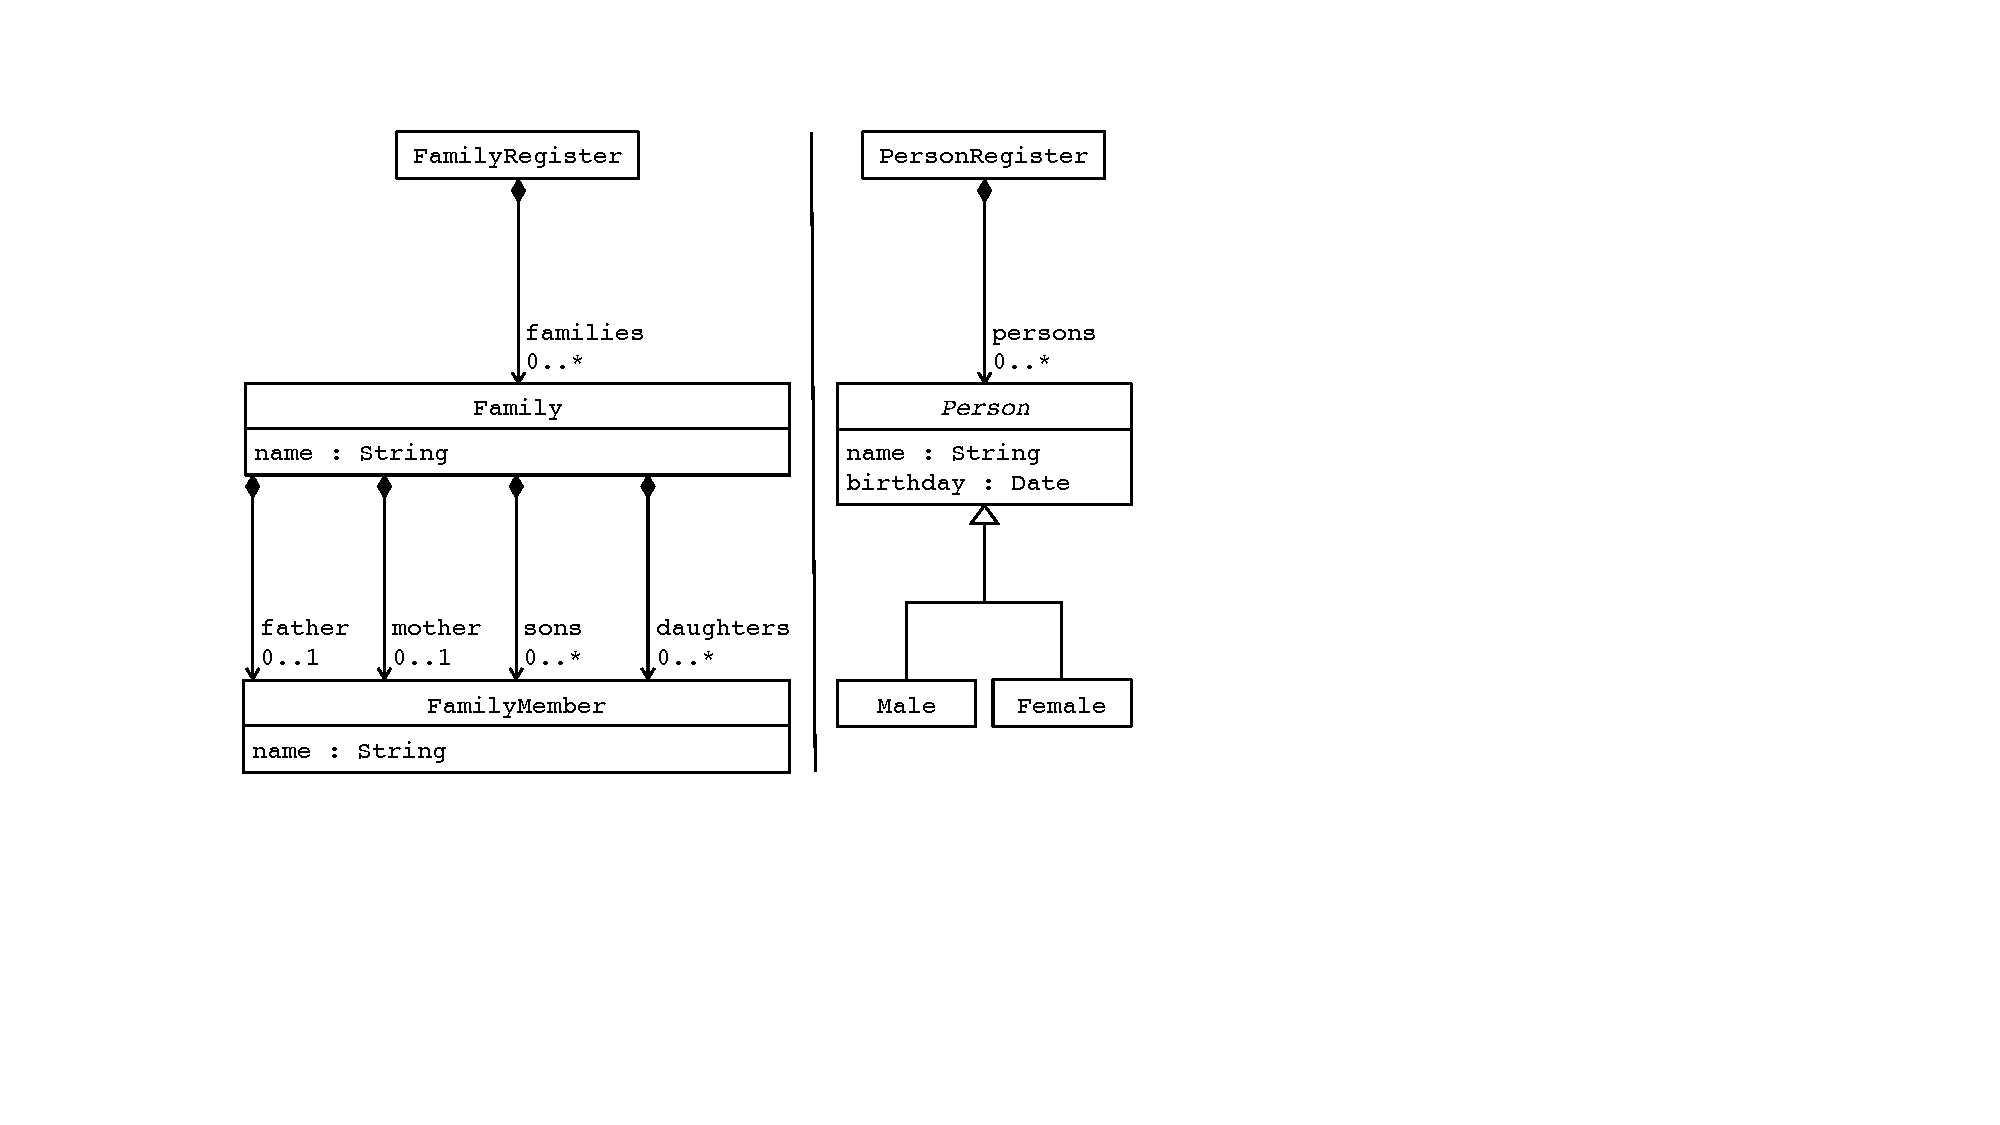
\includegraphics[width=\columnwidth]{diagrams/f2p-case/Metamodels}
	\caption{Metamodels}
	\label{fig:metamodels}
\end{figure}

\begin{figure*}[tb!]
	\centering
	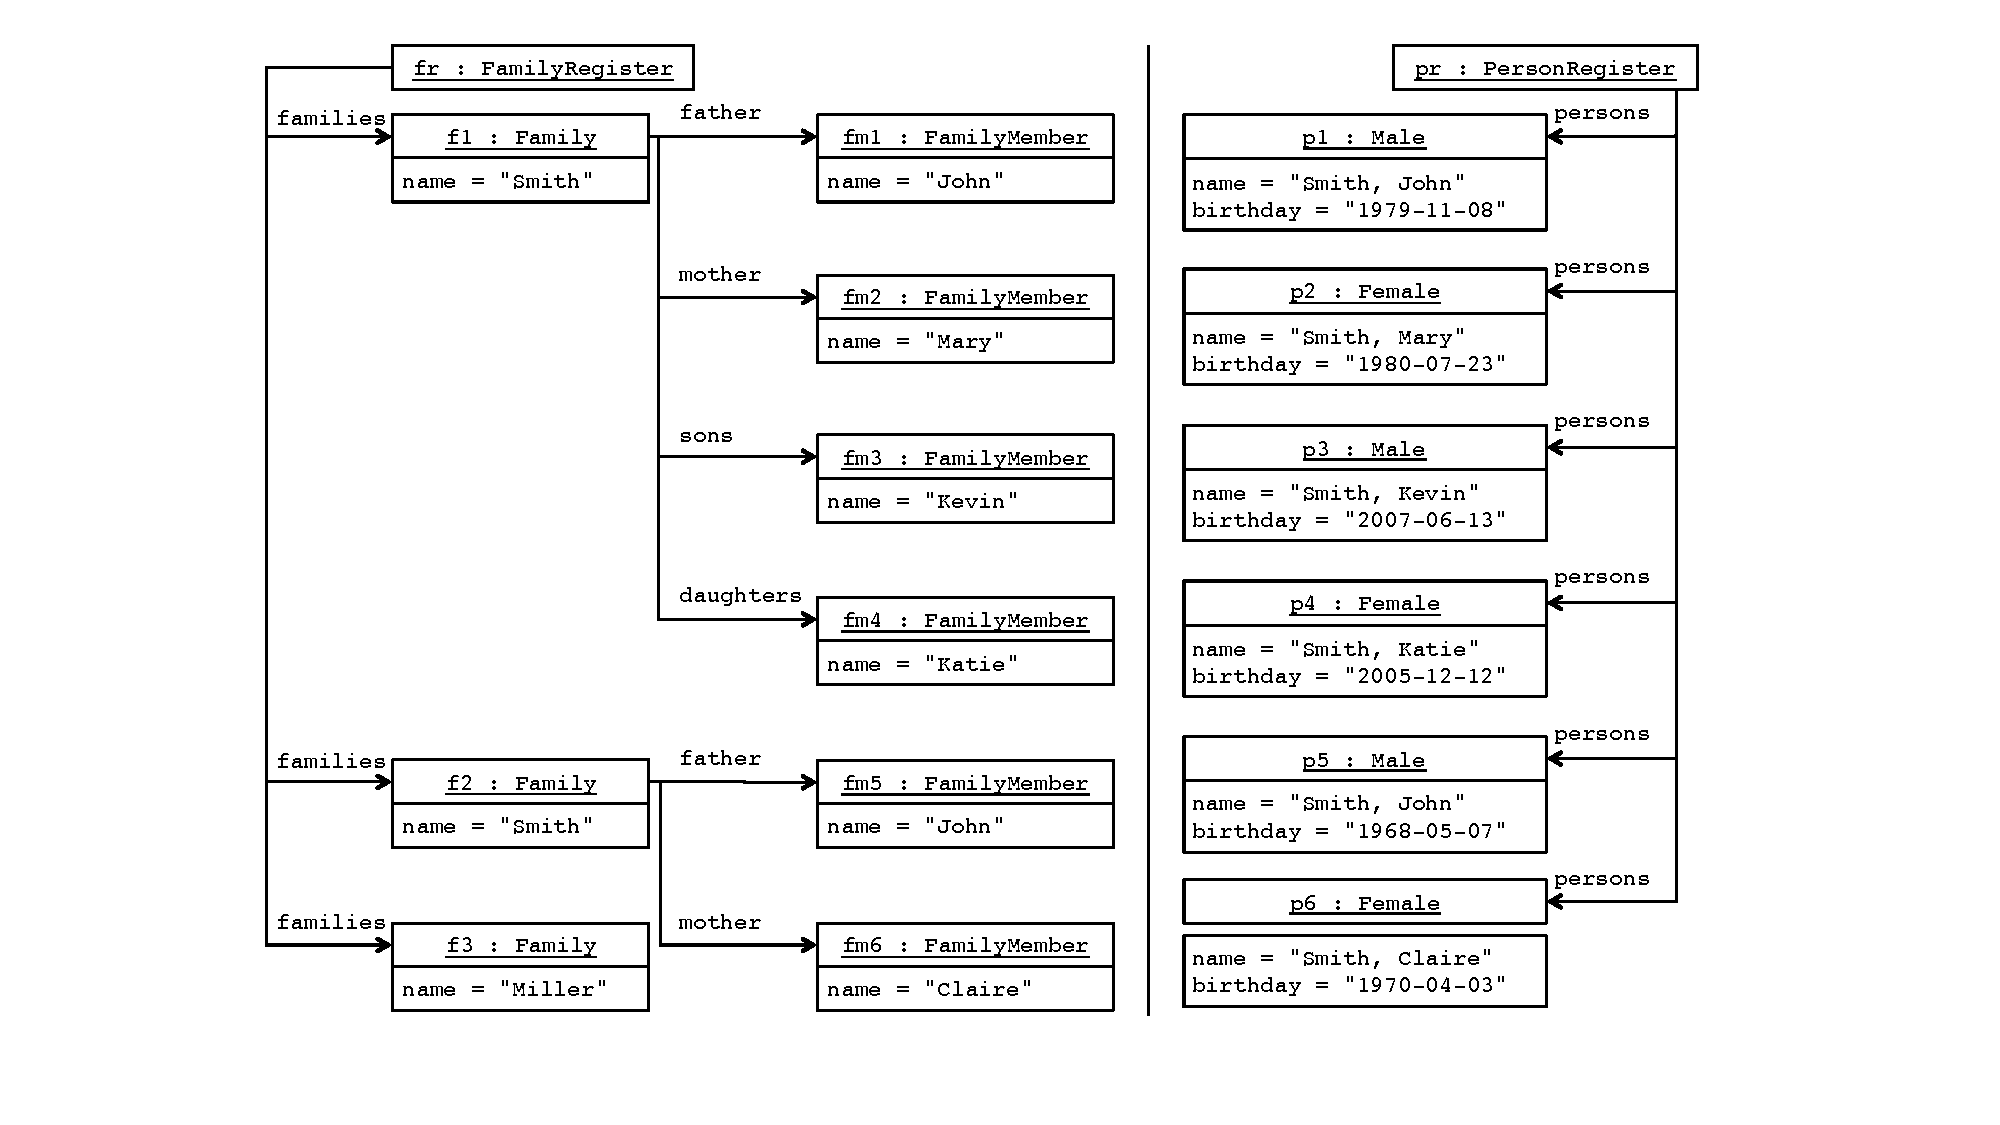
\includegraphics[width=0.75\textwidth]{diagrams/f2p-case/Models}
	\caption{Example of mutually consistent models}
	\label{fig:models}
\end{figure*}

We assume a unique root in each model (a family and a person register, respectively). 
A family register stores an unordered collection of families. 
Each family has members who are distinguished by their roles. 
The metamodel permits at most one mother and at most one father as well as an arbitrary number of daughters and sons. 
A person register maintains a flat unordered collection of persons who have a birthday and are either male or female. 
Note that key (combinations of) properties cannot be assumed in either model: There may be multiple families with the same name, family members with the same name even within a single family, and multiple persons with the same name and even the same birthday. 

A families model is \emph{consistent} with a persons model if a bijective mapping between family members and persons can be established such that:

\begin{enumerate}
	\item  Mothers and daughters (fathers and sons) are paired with females (males).
	\item  The name of every person $p$ is ``$f.name$,~$m.name$'', where $m$ is the member (in family $f$) paired with $p$.
\end{enumerate}

An example of mutually consistent models, conforming to the metamodels in figure~\ref{fig:metamodels}, is depicted as an object diagram in figure~\ref{fig:models}. 
%
The \emph{consistency relation} between families models and persons models is \emph{non-deterministic} in both directions: For a given families model, there are multiple consistent persons models (birthdays may be chosen arbitrarily). 
Conversely, a given persons model is consistent with multiple families models (due to different groupings into families and different roles, e.g., a female person can correspond to either a mother or daughter).

\subsection{Synchronization}
\label{sec:ConsistencyRestoration}

\subsubsection{Properties of synchronization}

The Families-to-Persons case is \emph{symmetric}~\cite{DBLP:journals/jss/DiskinGWC16}, i.e., neither model is a strict view of the other and information loss may occur in both transformation directions. We consider only \emph{directed synchronization}, assuming that changes have been applied to the master model, while the dependent model has not been changed at all or the changes do not affect the consistency relation (e.g., changes of birthdays in the persons model are allowed). 

We cover both \emph{batch synchronization}, where the dependent model is created from scratch, and \emph{incremental synchronization}, where the dependent model is changed to maintain consistency with the master model. 
Finally, changes are provided to the tools indirectly via an ordered\footnote{The results of some test cases depend on the order of elementary change operations.} sequence of change operations referred to as \emph{edits}.
%
These properties describe how the benchmark is designed but do not, however, prescribe the architecture of a bx tool that can be used to implement the benchmark (see section~\ref{sec:Foundations}).
For example, a bx tool can apply the provided edits and decide either to record operational deltas, structural deltas, or just to use only the old and new versions of the model.

\subsubsection{Bx laws}
\label{sec:BxLaws}

For the purpose of benchmarking, all bx laws are considered as \emph{properties} which may be satisfied or not. 
We test whether these laws hold for two reasons: First, a specific bx tool may not be designed to guarantee a certain bx law. 
Second, even if the tool has been designed to guarantee some law, its implementation may still contain faults, resulting in failing test cases.

From the bx  laws introduced in section~\ref{sec:Consistency}, the benchmark takes \emph{correctness} into account by the design of the test cases: All test cases check for consistency by requiring a dependent model which is consistent with the master model. Similarly, \emph{termination} and \emph{completeness} are considered implicitly as a violation of these properties would result in failing test cases. Finally, a few test cases of the benchmark explicitly address \emph{hippocraticness} by performing updates that do not affect consistency, respectively, to the master model. 

Several variants of \emph{round-trip laws} have been proposed in the literature.
In the symmetric bx case considered in the Families to Persons benchmark, two round-trip laws are required to hold: If the backward (forward) transformation is executed immediately after the forward (backward) transformation, the source model (target model) must not be changed.
These laws are not tested explicitly because they are implied in the case of correct and hippocratic synchronizers.

In the design of all test cases, we generally assume \emph{compositionality} of changes: The effect of the synchronization of a composite change is reduced to the composition of the effects of elementary changes. This corresponds to the \emph{put-put law} for delta lenses, as introduced in \cite{JOT:issue_2011_01/article6}. Furthermore, we take the principles of \emph{least change} and \emph{least surprise} into account.

Unfortunately, the expected behavior of a synchronizer may not be derived in a unique way by applying bx laws. In particular, this applies to the backward transformation, which is highly non-deterministic. To resolve non-determinism (which considerably complicates automatic testing and often is not desirable in practice anyway), we describe the expected behavior explicitly and uniquely, taking bx laws into account. The description is informal, yet (hopefully) precise (see below). 


\subsubsection{Synchronization behavior}      

In the following, we discuss the expected synchronization behavior for a series of ``small'' changes grouped according to model element (family, family member, person, \ldots) and then according to a limited set of change types (create, delete, update, move).
This overview is sufficient to provide a high-level intuition for the benchmark.
The actual test cases of course combine different changes and are more involved. However, the behavior of composite changes is \emph{induced} by the behavior of elementary changes (see above).

\paragraph{Forward synchronization:}

In the forward direction, the persons model must be manipulated to be consistent with the changed families model.
Defining the expected synchronization behavior is straightforward because the families model is determined uniquely, with the exception of birthday attributes.
To resolve non-determinism, we require that a default value be assigned as the birthday of a newly created person.
With this resolution, forward synchronization is deterministic.

\medskip
\noindent Changes to \emph{families} should be processed as follows:

\begin{description}
    \item[\textbf{Creation:}]
    New families can be created and must be inserted into the family register.
    This has no effect on the target model, which should not be changed.
    
    \item[\textbf{Deletion:}]
    A family can be deleted together with all its family members.
    All persons corresponding to the deleted family members should be deleted.
    
    \item[\textbf{Update:}]
    A family can be renamed.  All persons corresponding to the family members in the renamed family should be renamed accordingly.
    
    \item[\textbf{Move:}]
    Families cannot be moved as there is only a single family register and the collection of families is unordered.
\end{description}

\noindent Changes to \emph{family members} should be processed in the following manner: 

\begin{description}
    \item[\textbf{Creation:}]
    New family members can be created and must be immediately added to a family.
    A new person of the same gender as the family member should be created and added to the person register.
    The person's name should be appropriately composed from the family member's name and surname.
    The birthday of the person should have a default value (arbitrarily fixed by the benchmark). 
    
    \item[\textbf{Deletion:}]
    A family member can be deleted.  The corresponding person in the person register should be deleted.
    
    \item[\textbf{Update:}]
    A family member can be renamed.  The corresponding person should be renamed accordingly.
    
    \item[\textbf{Move:}]
    If a member is moved (defined as the combined deletion and creation of the link connecting the family member to a family), different cases have to be distinguished.
    If the gender of the family member is retained, the corresponding person object should be preserved; otherwise, the person should be deleted, and a new person with a different gender is created whose attributes are copied from the old person. 
    
    A move within a family does not affect the corresponding person's name; a move to another family results in a potential update of the person's name.
\end{description}


\paragraph{Backward synchronization:}

In the backward direction, a person may be mapped either to a parent or a child, and persons may be grouped into families in different ways. As argued earlier, non-determinism should be resolved as far as possible. This may be achieved in different ways. A \emph{default transformation} would fix specific mapping options (e.g., all persons may be mapped to children and grouped into the same family if their family names agree). 

To provide for more flexibility, we decided to require a \emph{configurable} backward synchronization, to be controlled by an \emph{update policy}\footnote{In practice this could either represent run time user interaction or compile time design preferences.} that must set two Boolean parameters:
(i) \code{prefer\-Parent\-To\-Child} controls whether a person is to be mapped to a parent or a child (if both options are possible), and (ii) \code{prefer\-Existing\-To\-New\-Family} determines whether a person is to be mapped to a family member added to an existing family, or added to a newly created family containing only this single family member (again if both options are possible). 
If both parameters are set to true, the second parameter should take precedence: If the only existing family with a matching family name has no unoccupied parent role, the member is inserted into the family as a child (thus respecting (ii) and ignoring (i)).

It should be noted that the update policy does not resolve non-determinism completely.
For example, let us assume that persons should be added to existing families as children.
If we insert another person with family name \code{Smith} into the persons model depicted in figure~\ref{fig:models}, a corresponding member may be inserted either into family \code{f1} or into \code{f2}.
Furthermore, the update behavior may depend on the \emph{order} of change operations. For example, if persons should be added to existing families as parents, and two male persons with family name \code{Miller} are added to the persons model, the first person will be added as a father and the second person as a son. 

\medskip
\noindent Let us now consider change operations on \emph{persons}:
%
\begin{description}
    \item[\textbf{Creation:}]
    New persons can be created and must be added to the person register.
    A new family member with correct gender and name should be created in a suitable family in the family register.
    The update policy is consulted if it is possible to add the new family member to an existing family, and if the family member can be added as a parent or a child.
    
    \item[\textbf{Deletion:}]
    Persons can be deleted.
    The corresponding family member should be deleted. 

    \item[\textbf{Update:}]
    Changes of birthdays do not affect the families model. 
%
    The first name of a person can be changed; 
    the name of the corresponding family member should be updated accordingly. 
%
    The family name of a person can be changed; 
    this change should not affect the current family and its members.
    The family preserves its name even if it does not contain any other members.
    The corresponding family member should instead be moved to another family, which may have to be created as required; the precise update behavior, if there are multiple possibilities, depends on the specified update policy for the particular test case.
    
    \item[\textbf{Move:}]
    Persons cannot be moved because the persons model consists of a single, flat, unordered collection. 
\end{description}

The update policy constitutes an example of \emph{ap\-pli\-ca\-tion-specific requirements}, as discussed at the end of section~\ref{sec:BxLaws}. The rules for handling changes to family names are application-specific, as well. They are based on the underlying assumption that the person intends to leave their family (e.g., because of marriage).
This kind of synchronization behavior may (arguably) be considered reasonable; we simply take it for granted, being required by an (imaginative) customer.
However, in certain circumstances it may (arguably) violate principles such as least change (e.g., if the person was the single member of a family); we use these principles only as general guidelines, not as strict laws. 


\subsection{Challenges}
\label{sec:Challenges}

The Families-to-Persons case includes a number of diverse \emph{challenges} summarized in the following:

\begin{description}
	\item[\textbf{Heterogeneous metamodels:}] 
	Solutions must establish a mapping between heterogeneous metamodels, where the same information is represented in different ways (concerning, e.g., names and genders).
	
	\item[\textbf{Loss of information:}] 
	The scenario is symmetric as the family structure is only present in the source, and birthdays are only present in the target.
	
	\item[\textbf{No keys:}] 
	There are no uniquely identifying (combinations of) properties for family members or persons, which makes synchronization difficult.
	
	\item[\textbf{Non-determinism:}] 
	The consistency relation is not de\-ter\-mi\-ni\-stic: For a given families model, there can be multiple correct persons models (birthdays may be arbitrarily selected). 
	Likewise, for a given persons model there can be multiple correct families models (due to different groupings into families and different roles in these families). Synchronization has to deal with this non-determinism (and resolve it as far as possible).
	
	\item[\textbf{Configurability:}] 
	The behavior of backward synchronization is controlled by an update policy determining roles of members and groupings of members into families. 
	The update policy may be changed at run time and should take effect only for future updates (there is to be no global reshuffling of the families model after the update policy has been changed).
	
	\item[\textbf{Renaming and movement:}] 
	Changes to be synchronized include not only creations and deletions, but also renamings and moves, which must not be reduced to deletions and creations so that changes can be synchronized in a minimally invasive way. 
	
	\item[\textbf{Order-dependent synchronization:}] 
	Backward synchronization depends on the order in which change operations on the persons model are processed. 
	For example, if two persons of the same gender are to be inserted into the same family as parents, only the first person can be inserted as a parent; the second person must be added as a child.
	
	\item[\textbf{Specific least surprise requirements:}]~
	The bench\-mark requires adherence to an application-specific definition of what ``least surprise'' is to mean.
	For example, if the family name of a person is changed, the corresponding family member should be moved to another family (rather than having the family name updated, with possible side effects on other members).
	This definition of which change is ``better'' or ``smaller'' than another is arguably arbitrary and must be treated as an additional requirement.
\end{description}
%%% Local Variables:
%%% mode: latex
%%% TeX-master: "../main"
%%% End:
